% !TeX spellcheck = en_EN-English

\section{Embedding of Patient}
\label{embedding}

First of sub-tasks for prediction of patient future costs is to embed each patient record into numerical vector that would be understandable for neural network. Our main goal was to create embedding that retain similarity information, meaning that records for similar diagnosis, drugs and medical procedures would receive similar embedding where we define similarity by the Euclidean distance between embedding vectors. Retaining similarity is important for in order to make prediction task of predicting future records easier for model since it would be sufficient to predict just closely related record and not necessary exact one. 
\\

For each record of a patient we embed four information. First and easy to implement is a timestamp which is computed using numerical and date values, then there are three more tricky information and those are diagnosis, medical procedure and prescribed drug. 

\subsection{Timestamp}

Attribute what we call timestamp of patients record can more precisely described as approximation of patients age at the moment of either medical procedure or drug prescription. This timestamp is computed using two of available information and those are age of patient in years and date of record. The specific procedures we use compute this timestamp can be found in section \ref{timespampImple}, in general we find first record, compute timestamp based on patient age as approximate age in days at that point and then compute subsequent timestamp as timestamp of first record plus difference of record dates. This way each timestamp contains approximation of age of patient while also containing information about order of records and comparative timeframe between each two records.

\subsection{Diagnosis embedding}
\label{diagEmb}

Base diagnose information we embed was ICD-10-CM code of disease.ICD-10-CM stands for "International Classification of Diseases, Tenth Revision, Clinical Modification" and is used to code and classify medical diagnoses \cite{cdcICD10CM} most precisely version of this code that is used in Slovakia and is better known by the acronym MKCH-10-SK (Medzinárodná klasifikácia chorôb) \cite{ncziMKCH}.\\

\begin{figure}[!h]
	\centering
	
	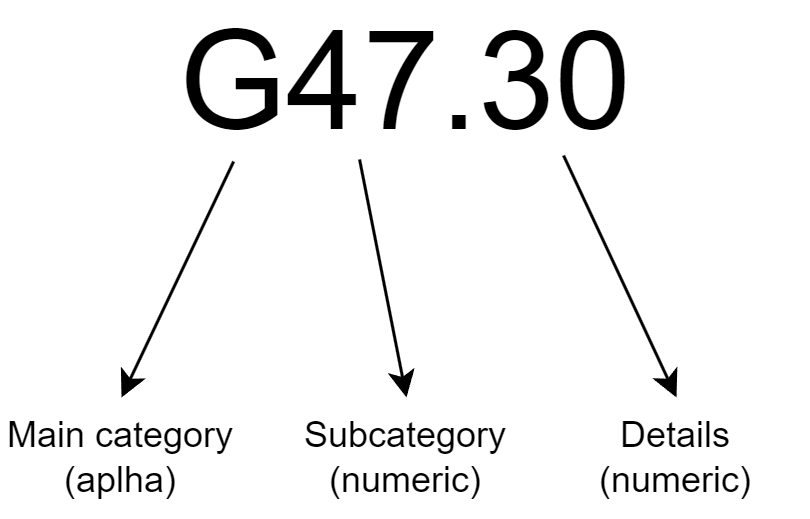
\includegraphics[width=0.8\textwidth]{images/ICD-10-CM.png}
	
	\caption{Structure of MKCH-10 code.}
	\label{fig:icd-10-cm}
\end{figure}

This code consist of three parts as shown on Fig. \ref{fig:icd-10-cm}. First part is one letter that encodes main categories of diseases also known as chapter, for example codes starting with G are diseases of the nervous system. 
After that there is two numeric characters that further specify subcategory of disease such as codes from G40 to G47 which are episodic and paroxysmal disorders and specifically G47 are sleep disorders. 
We can see that episodic and paroxysmal disorders are only up to G47, meaning that theoretically there can exist subgroups G48 and G49 which have 4 in second position but does not belong to same G4 subcategory as G40 or G47 \label{mkch_subdiv}. Thankfully this is not the case and in cases like this when higher lower subcategory (like G4) does not have 10 lower level subcategories (like G47) these subcategories does not exist at all and in case it have more than 10 lower level subcategories it gets multiple consecutive high level subcategories, for example disorders of other endocrine glands spans from E20 to E35. 
Then code contains dot after which there are characters that further describe details of disease such as etiology, anatomic site and severity. Official documentation of ICD-10-CM codes stands that codes can be up to 7 characters long meaning that after first three characters specifying category there can be up to 4 alphanumeric to further specify the disease \b{CITE}, however Slovak version MKCH-10 codes contains at most two numeric characters to specify disease \b{cite} and these details are organized in a way where the first position conveys higher-level information than the second, for example G47.3 is sleep apnea and G47.30 is primary central sleep apnea.
\\

To embed this code we firstly split it into it's three parts and embed each part separately. After that we concatenated embedding of each part to get final embedding of disease.
To embed main category we generated vector containing random numbers from uniform distribution for each letter of English alphabet (all main categories). We used random vectors in order to have relatively similar distance between any two main categories since there are no particular relationships between these categories, we were thinking also about using one-hot encoding which would make distance between each two categories perfectly same but we didn't do it since it would have restricted length of vector. 
\\

In embedding second part which is subcategory we used different approach, where to each number between 00 and 99 (all possible values of this part) we assigned linearly number in chosen interval. This assigned number was then repeated multiple times to create vector. This approach has advantages and disadvantages. Advantage is that we can be sure that closely related disease subgroups like G46 and G47 would get close embedding since their subgroup codes are close on number line. However there are also two disadvantages, first is that G49 and G50 would be similarly close as G46 and G47, but thankfully in a most cases either X9 code doesn't exist at all, creating a gap, or if X9 code exist it belong to category that go past X on as higher level subgroup. Another disadvantage is that distance between two higher level subgroups can vary quite dramatically even though in reality there might not be reason for that difference in distance. For example, using this approach higher level subgroup G40-G47 is much closer to subgroup G50-G59 than to G80-G83.
\\

Finally to embed details we decided to use same approach as for subgroups since these codes work similarly, only difference was that not all codes had second level details, in such cases we add 5 as a proxy in order to minimize average distance from all potential codes with same first level details code that contain second level detail information while also maximizing average distance to different first level detail codes.
\\

Once all parts are embedded we can create final embedding as their concatenation, to encode importance of each part in final embedding we gave them different lengths, this works thanks to the fact that each value in each of vector have same mean and same variance. 
Importance of each level was encoded using different lengths of vector for each part where embedding of main category was longest and details got shortest embedding.

\subsection{Drug embedding}
\label{drugEmb}

Similarly to diagnosis, to embed drug information we embed international code associated to these drug. In case of drugs it was Anatomical Therapeutic Chemical classification system also known under abbreviation ATC. In a same way as MKCH-10 code this code can be split into multiple parts where each next part contains finer information. It contains of 5 parts or levels. First level encodes main anatomical or pharmacological groups. There are fourteen such groups, encoded by single letter, which are shown in the Fig. \ref{fig:atc_l1}. Then second level encodes pharmacological or therapeutic subgroup using two digit number, after that there two levels that further specify pharmacological, therapeutic or even chemical subgroup, these two levels are both encoded using single letter each. Final fifth encoded with two digit number contains information about specific chemical substance inside drug.

\begin{figure}[!h]
	\centering
	
	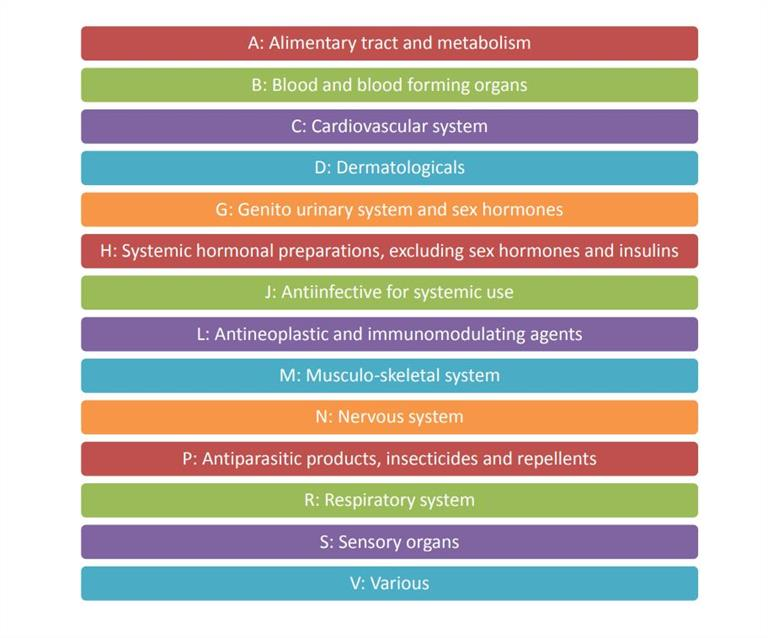
\includegraphics[width=0.8\textwidth]{images/atc_l1_classification_who.jpg}
	
	\caption{Fourteen main anatomical or pharmacological groups and their corresponding first level ATC code \cite{atc_who}.}
	\label{fig:atc_l1}
\end{figure}

Embedding was done in very similar way as in diagnosis embedding, meaning each level was embedded separately and final embedding was done as concatenations of them. In this case each level was embed using random vector from uniform distribution. We used random vectors for each level since none of levels contains any internal sub-groupings similar to subgroups of diagnosis (see \ref{mkch_subdiv} subgroup codes). To encode importance of levels we again used lengths of random vectors. With this embedding we should get codes whose similarity is more dependent on whether lower more important levels match than higher ones.
\\


\subsection{Medical procedure embedding}
\label{procedureEmb}

Final part to embed was medical procedures. In this case there is no structured code that can be used and is implemented in Slovak healthcare systems. So what we have done is to embed description of the procedures. For that we tried two different approaches, first was large language model (LLM) trained on multiple languages including Slovak and second was Word2vec model, explained in section \ref{theoryW2v}, specific for Slovak language. Dimensionality of resulting embedding was then reduced using PCA, to get rid of dimensions with small variance meaning they encode small amount of information. 
\\

For LLM we specifically choose LaBSE model which we explained in section \ref{theoryLaBSE}, since this model is trained to give similar embedding to similar sentence regardless of language in which sentences are, we hoped that thanks to this approach we would get better embedding of procedure description that contains professional medical terms which are a lot of times international and might not be part of corpus for model trained on single language.
\\


Finally we create record embedding by concatenating all four parts. Since we have two separate datasets, one for prescribed drugs and one for medical procedures, we always have only three out of four information available for each record, since timestamp and diagnosis are always available, we substitute missing part with vector of zeros with appropriate length which is most neutral embedding since we centered both medical procedure and drug prescription embedding around zero.
